\documentclass[12pt]{book} % Possui capítulos, título e resumo ocupam página toda, 2-sided, inclui header com # da pág, capítulo e seção.

\usepackage{graphicx}                            % Para poder incluir gráficos.
\usepackage{natbib}                              % \citep{jon90} --> (Jones et al., 1990)
\usepackage{amssymb}                             % Para poder utilizar alguns símbolos matemáticos especiais.
\usepackage[usenames,dvipsnames]{color}          % Para ampliar a quantidade de cores utilizáveis.
\usepackage[colorlinks,citecolor=Blue,linkcolor=BrickRed]{hyperref} 
\usepackage[nottoc]{tocbibind}                   % Para incluir referências bibliográficas no sumário.
                                                 % Para colocar links nas referências, equações, figuras, etc, além de menu árvore no PDF.

%%% Formatação %%%
\usepackage[small,bf]{caption}                   % Para que legendas de figuras e tabelas fique em fonte menor e com negrito.
\usepackage{fancyhdr}                            % Para poder fazer cabeçalhos e rodapés mais bonitos.
\usepackage{mathptmx}                            % Para mudar a fonte usada na matemática para uma mais parecida com times. 
\usepackage{helvet}                              % Para que a fonte não-serifada seja Helvetica.
\usepackage{titlesec}                            % Para mudar a formatação dos títulos dos capítulos e seções.
\titleformat{\chapter}[display]
  {\normalfont\sffamily\Large}
  {\chaptertitlename\ \thechapter}{10pt}{\LARGE\bfseries}
\titleformat*{\section}{\Large\sffamily\bfseries\raggedright}
\titleformat*{\subsection}{\large\sffamily\bfseries}
\titleformat*{\subsubsection}{\normalsize\sffamily\bfseries}

\newcommand{\Tstrut}{\rule{0pt}{2.3ex}}          % = `top' strut
\newcommand{\xline}{\hline\Tstrut}               % Linha de tabela com mais espaço
\usepackage{dcolumn}                             % Para alinhar números em tabelas pela vírgula
\newcolumntype{d}[1]{D{.}{,}{#1}}                % Para alinhar números em tabelas pela vírgula
\newcommand{\nt}[1]{\multicolumn{1}{r}{#1}}      % Para colocar coisas sem vírgula na tabela
\newcommand{\ctit}[1]{\multicolumn{1}{c}{#1}}    % Para colocar títulos na tabela com dcolumn

\newcommand{\dd}{\mathrm{d}}                     % Para o 'd' de diferencial não ficar em itálico.
\newcommand{\nv}[1]{\mathrm{#1}}                 % Para abreviar o formato mathroman. 
\newcommand{\la}{\lesssim}                       % Abreviação de menor que aprox.
\usepackage{mathtools}                           % To use dcases environment in equations.

\newenvironment{alltt}{\ttfamily}{\par}
\usepackage{moreverb}
\usepackage{caption}


% Define as bordas do documento
\usepackage[a4paper, top=2.5cm, bottom=3.5cm, inner=3.0cm, outer=3.0cm]{geometry}

% Redefinindo estilo da página de início de capítulo
\fancypagestyle{plain}{
\fancyhf{}                                           % Limpa definições anteriores.
\fancyfootoffset{0cm}                                % Estica o rodapé pra fora das margens.
\fancyfoot[LE,RO]{\footnotesize \thepage}            % Número da página nas quinas e em negrito.
\renewcommand{\headrulewidth}{0pt}                   % Tira linha do cabeçalho.
\renewcommand{\footrulewidth}{0pt}}                  % Tira linha do rodapé.
\pagestyle{fancy}                                    % Define estilo das outras páginas.
\fancyhf{}                                           % Limpa definições anteriores.
\fancyhead[LE]{{\sffamily \scriptsize \leftmark}}    % Capítulo na esquerda.
\fancyhead[RO]{{\sffamily \scriptsize \rightmark}}   % Seção na direita.
\fancyfootoffset{0cm}                                % Estica o rodapé pra fora das margens. 
\fancyfoot[LE,RO]{\footnotesize \thepage}            % Número da página nas quinas e em negrito.

\let\origdoublepage\cleardoublepage                  % Para deixar em branco páginas sem conteúdo 
\newcommand{\clearemptydoublepage}{%
  \clearpage
  {\pagestyle{empty}\origdoublepage}%
}
\let\cleardoublepage\clearemptydoublepage            % Fim do deixar em branco páginas sem conteúdo

% Para capa fancy
\newcommand{\lyxline}[1][1pt]{
  \par\noindent
    \rule[.5ex]{\linewidth}{#1}\par}

%%% Começo do documento %%%
\begin{document}

%--------------------Página de rosto------------------------%
\begin{titlepage}                                                 
\begin{center}
%\vspace{12cm}
{\Huge \sffamily \bfseries FLASK:\vspace{0.5cm}\linebreak 
Full-sky Lognormal Astro-fields Simulation Kit}\\
\vspace{1cm}
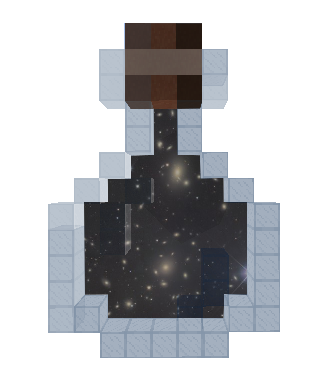
\includegraphics[width=0.6\textwidth]{flask_logo.eps}\\
\vspace{1cm}
{\LARGE \sffamily Usage and installation manual}
\end{center}
\vspace{1.5cm}
\begin{flushright}
\begin{minipage}[c][1\totalheight][t]{9 cm}
\lyxline{\normalsize}
\vspace{0.2cm}
\textbf{Written by:} Henrique S. Xavier\\
\textbf{Contact:} {\tt hsxavier@if.usp.br}\\
\linebreak
University College London, UK\\
Universidade de S\~{a}o Paulo, Brazil
\vspace{0.2cm}
\lyxline{\normalsize}
\end{minipage}
\par\end{flushright}
\vspace{1cm}
\begin{center}
{\normalsize\today}
\end{center}
\end{titlepage}
%-----------------------------------------------------------%
\newpage
\thispagestyle{empty}

% Índice
\tableofcontents

% Começo de verdade da monografia 

\chapter{Disclaimer}
\label{sec:disclaimer}

   {\sc flask} is free software, written by Henrique S. Xavier; 
   you can redistribute it and/or modify it under the terms of the GNU 
   General Public License as published by the Free Software Foundation; 
   either version 2 of the License, or (at your option) any later version.

   {\sc flask} is distributed in the hope that it will be useful,
   but without any warranty; without even the implied warranty of
   merchantability or fitness for a particular purpose. See the
   GNU General Public License for more details. You should have received 
   a copy of the GNU General Public License along with {\sc flask}; if not, 
   write to the Free Software Foundation, Inc., 59 Temple Place, Suite 330, 
   Boston, MA  02111-1307  USA.

   Thank you for using this software. Please report any bugs to {\tt hsxavier@if.usp.br} and
   acknowledge {\sc flask} by citing the publication \citet{Xavier16mn}.
   

\chapter{Installation}
\label{sec:installation}

\section{Requirements}
\label{sec:requirements}

{\sc Flask} is a code written in {\sc C++} that uses {\sc OpenMP} for parallelization; 
{\sc healpix}\footnote{{\tt \href{http://healpix.jpl.nasa.gov}{http://healpix.jpl.nasa.gov}}} for 
mapping the sky and performing harmonic transforms; the Gnu Scientific 
Library\footnote{{\tt \href{http://www.gnu.org/software/gsl}{http://www.gnu.org/software/gsl}}} 
({\sc GSL}) to generate pseudo-random numbers, to perform Cholesky decompositions and other tasks; and the 
{\sc cfitsio}\footnote{{\tt \href{http://heasarc.gsfc.nasa.gov/fitsio}{http://heasarc.gsfc.nasa.gov/fitsio}}} 
library to input and output FITS files. Apart from {\sc healpix}, all the remaining dependencies should 
be available on Linux and Mac repositories. {\sc Healpix} however should be easy to install (just 
follow their instructions); {\sc Flask} requires version 3.11 or later of the C++ {\sc healpix} 
implementation due to specific functions implemented only on these versions. 

So far {\sc Flask} has been tested only on Linux distributions -- Scientific Linux 5.6 and Ubuntu 14.04 -- 
and compiled with {\tt g++} (GCC) versions 4.8.1 and 4.8.4.   
Besides the main code and other routines in {\sc C++}, {\sc flask} also includes auxiliary {\sc python} 
and {\sc shell} scripts. These were tested in {\sc bash} shell and {\sc python} versions 2.7.3 and 2.7.6. 
The {\sc python} scripts require the a few packages like {\sc numpy}, {\sc scipy} and {\sc healpy} 
(which can be installed by following {\sc healpix} instructions). Check the scripts for further dependencies.  

\section{Compiling}
\label{sec:compiling}

Before compiling, you will have to modify the {\tt Makefile} in the {\tt src} sub-directory of {\sc flask}. 
The following lines must be changed according to the location of the {\sc healpix} installation directory:

\vspace{0.5cm}

\noindent
{\tt HEALDIR = <path to Healpix directory>}

\noindent
{\tt CXXHEAL = -I<path to Healpix header files>}

\noindent
{\tt LDHEAL  = -L<path to Healpix library files>} 
\vspace{0.5cm}

\noindent
In case other libraries such as {\sc cfitsio}, {\sc gsl} are installed in non-standard locations, 
you might need to specify their locations with similar compiler flags. The default compiler in the 
{\tt Makefile} is {\tt g++}, you might need to change the keyword {\tt COMP} as well if using a 
different compiler.

After changing the {\tt Makefile}, run the command {\tt make} in the {\tt src} directory. The 
executables will be built in {\sc flask} {\tt bin} sub-directory. You may add this sub-directory to 
your {\sc path} environment variable in order to be able to run {\sc flask} anywhere; otherwise, 
you will require to run it from there or to provide the full path as usual. 


\chapter{Usage}
\label{sec:usage}

\section{Using {\sc flask}}
\label{sec:flask}

\subsection{Quick start}
\label{sec:quick-start}

To get a feeling of {\sc flask} and to test if things are working fine, go to the {\sc flask} 
directory and run the command:

\vspace{0.5cm}
\noindent
{\tt ./bin/flask example.config}
\vspace{0.5cm}

\noindent
This should result in a clean run (no errors or warnings) and should make {\sc flask} 
use typical data stored in the {\tt data} sub-directory to create 
the most relevant outputs into the {\tt example} sub-directory (which should be empty), 
including maps and catalogs simulations. Since writing files to the hard-disk is a slow process, 
this run will take much longer than an usual {\sc flask} run that only outputs one or two files. 
To figure out what the output files are, check the file {\tt example.config} and Sec. 
\ref{sec:keywords}.
 
\subsection{Basic operation}
\label{sec:operation}

{\sc Flask} is executed through the command line, and it always requires a configuration file 
(e.g. {\tt example.config} in the {\sc flask} directory):

\vspace{0.5cm}
\noindent
{\tt flask <config file>}
\vspace{0.5cm}

Any keyword in the configuration file can be altered from the command line by specifying its 
name {\tt<keyword\_i>} and value {\tt<value\_i>} after passing the configuration file to {\sc flask}: 

\vspace{0.5cm}
\noindent
{\tt flask <config file> <keyword\_1>: <value\_1> <keyword\_2>: <value\_2>...}
\vspace{0.5cm}

\noindent
For example,

\vspace{0.5cm}
\noindent
{\tt flask example.config RNDSEED: 334 MAP\_OUT: ./map-002.dat}
\vspace{0.5cm}

{\sc Flask} outputs to the screen a comprehensive description of what it is doing. In case you want to 
store this information for later, you might want to redirect the output to a file, e.g.: 

\vspace{0.5cm}
\noindent
{\tt flask example.config RNDSEED: 334 MAP\_OUT: ./map-002.dat > r334.log}
\vspace{0.5cm}

\subsection{Inner workings}
\label{sec:workings}

The internal process followed by {\sc flask} is described in \citet{Xavier16mn}. 
Fig. \ref{fig:flow-chart} shows a flow chart that roughly described the 
operations sequences. Some processes are only performed when simulating lognormal 
fields (Gaussian simulations may skip a few of them). Other processes like 
creating triangular matrices used for generating correlated random variables and 
performing a density line-of-sight (LoS) integration to get the convergence are 
optional (they are executed according to the specifications in the configuration file).

\begin{figure}
  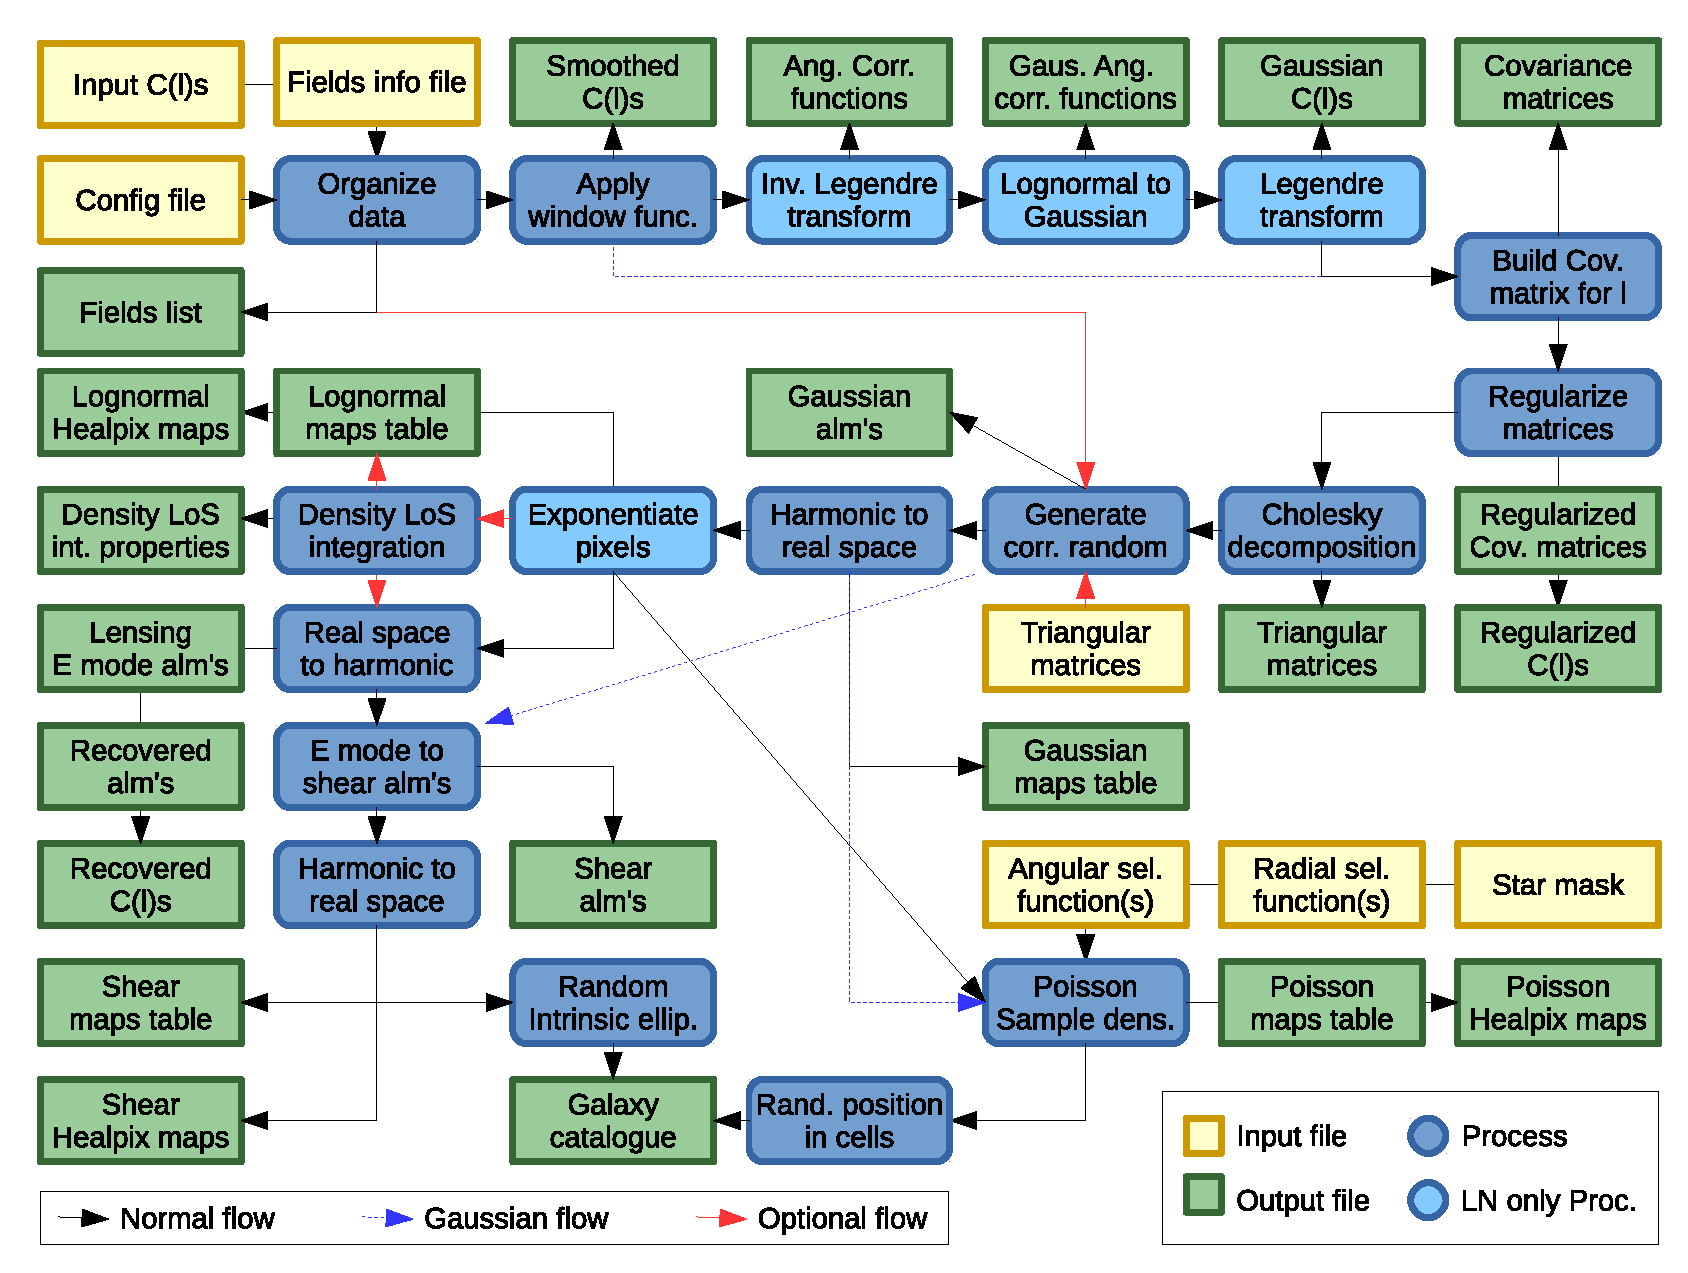
\includegraphics[width=1\textwidth]{flask_flow_chart.eps}
  \caption{{\sc Flask} basic flow chart.}
\label{fig:flow-chart}  
\end{figure}


\subsection{Configuration file keywords}
\label{sec:keywords}

{\sc Flask} is built in a way that all the existing keywords in the code must be present in the 
configuration file otherwise a warning message is issued; this is to avoid setting keywords to 
values unknown by the user and to disclose to the user all available options in the code. 
{\sc Flask} will also complain if keywords that do not exist in the code are present in the 
configuration file or are passed through the command line; keywords are identified by a colon (:) 
after it, so this should not be used for other purposes inside configuration files. Although 
the hash (\#) is used to identify comments, this is only for aesthetic reasons and does not have 
any effect on the parsing of the configuration file ({\tt \# DENS2KAPPA:} is still identified as 
the {\tt DENS2KAPPA} keyword). More information about this can be found in the {\tt example.config} 
file.

{\sc Flask} goes through a series of sequential computations that transforms the simulated data somehow; 
after each step, the code can output the current status of the data. These possible outputs are 
presented in the {\tt example.config} file in the exact order they are produced. Thus, one can 
have an idea of the simulation process by reading the output options in that file. All outputs 
can be turned off by assigning {\tt 0} to the respective keyword.

We now provide a description of every keyword available in the code (a brief description of 
each one is also provided in {\tt example.config}):

\begin{itemize}

\item {\tt DIST:} This takes as value one string that can be either {\tt GAUSSIAN}, 
  {\tt LOGNORMAL} or {\tt HOMOGENEOUS}, specifying what kind of distribution all 
  the simulated random fields will follow. The {\tt HOMOGENEOUS} in fact ignores 
  all input power spectra $C(\ell)$s as if they were all zero and creates homogeneous 
  field maps. Density fields can be later Poisson sampled according to the selection 
  function, so the {\tt HOMOGENEOUS} choice is useful to create the random catalogues 
  used in \citet{LandySzalay93x}, for instance. Weak lensing shear produced under this 
  choice is currently zero, and ellipticities are completely random according to 
  {\tt ELLIP\_SIGMA}. For simulating Gaussian and lognormal correlated fields 
  simultaneously, one should use the {\tt LOGNORMAL} choice and adjust the input 
  information so to approximate the desired fields to a Gaussian distribution.

\item {\tt RNDSEED:} This is a single integer number, the seed for the pseudo-random 
  number generator. In fact, the seed is transformed into $N_{\nv{proc}}$ seeds, where 
  $N_{\nv{proc}}$ is the number of processors available for parallel computing with 
  {\sc OpenMP}. This transformation is such that every seed provided to {\tt RNDSEED} 
  will result in different and exclusive set of $N_{\nv{proc}}$ so that different seeds truly 
  result in independent realisations. Note that a given seed passed to {\tt RNDSEED} will 
  only result in the same realisation as long as $N_{\nv{proc}}$ remains the same.

\item {\tt POISSON:} This can be {\tt 1} or {\tt 0}, and specifies if the galaxy density 
  fields should be Poisson sampled or not, respectively. If not sampled (useful for debugging 
  reasons), the value attributed to the {\sc healpix} map is the expected number of galaxies 
  (a non-integer number). This map can then be output through the {\tt MAPWER\_OUT} and 
  {\tt MAPWERFITS\_PREFIX} keywords. Generating a galaxy catalogue from this map (with 
  {\tt POISSON: 0}) would not make much sense and is likely to cause the code to crash.

\item {\tt OMEGA\_m:} This takes a real number that represents the total matter (dark matter 
  plus baryons) density parameter. It is only used if the user sets: (1) {\tt DENS2KAPPA: 1}; or 
  (2) {\tt SELEC\_TYPE: 1} or {\tt SELEC\_TYPE: 3}.

\item {\tt OMEGA\_L:} This takes a real number that represents the dark energy density parameter. 
  It is only used if the user sets: (1) {\tt DENS2KAPPA: 1}; or (2) {\tt SELEC\_TYPE: 1} or {\tt SELEC\_TYPE: 3}. 

\item {\tt W\_de:} This takes a real number that represents the $w_0$ parameter of a constant dark energy 
  equation of state. It is only used if the user sets: (1) {\tt DENS2KAPPA: 1}; or (2) {\tt SELEC\_TYPE: 1} 
  or {\tt SELEC\_TYPE: 3}. Currently this is the only kind of dark energy model implemented in the code. 

\item {\tt ELLIP\_SIGMA:} This takes a real number that represents the standard deviation of the zero mean 
  Gaussian distribution from which each component of the galaxy intrinsic ellipticity $\epsilon_{\nv{s}}$ 
  is randomly drawn. The final ellipticity in the catalogue is $\epsilon=\epsilon_1+i\epsilon_2$:
  \begin{equation}
    \epsilon = 
    \begin{dcases}
      \frac{\epsilon_{\nv{s}}+g}{1+g^{*}\epsilon_{\nv{s}}}, & |g|\leq 1; \\
      \frac{1+g\epsilon_{\nv{s}}^{*}}{\epsilon_{\nv{s}}^{*}+g^{*}}, & |g|>1;\\
    \end{dcases}
    \label{eq:ellipticity}
  \end{equation}
  where $g\equiv \gamma/(1+\kappa)$ is the reduced shear, $\gamma=\gamma_1+i\gamma_2$ is the shear, $\kappa$ is the 
  convergence, and $\epsilon_{\nv{s}}=\epsilon_{\nv{s},1}+i\epsilon_{\nv{s},2}$ is the galaxy intrinsic 
  ellipticity \citep[we follow ][eq. 4.12]{Bartelmann01mn}.
  
\item {\tt GALDENSITY:} This takes a real number representing the 3D comoving galaxy number 
  density in $(h^{-1}\nv{Mpc})^{-3}$. It is only used if {\tt SELEC\_TYPE: 1} or {\tt SELEC\_TYPE: 3}. 

\item {\tt FIELDS\_INFO:} This takes a string representing the path to the fields information file 
  described in Sec. \ref{sec:fields-info}.

\item {\tt CHOL\_IN\_PREFIX:} This takes the character {\tt 0} or a string representing the path, including 
  a file prefix, to the files written by the keyword {\tt CHOLESKY\_PREFIX} in a previous {\sc flask} run. If set to 
  {\tt 0}, the code: takes as input the power spectra $C_{\nv{in}}(\ell)$s specified by {\tt CL\_PREFIX}; 
  process it to obtain the associated Gaussian power spectra $C_{\nv{g}}(\ell)$s [if {\tt DIST: LOGNORMAL}, 
  otherwise $C_{\nv{g}}(\ell)=C_{\nv{in}}(\ell)$]; build independent covariance matrices for each $\ell$; 
  regularise the matrices if necessary and requested; and perform a Cholesky decomposition to obtain 
  triangular matrices -- which can be written to files by the {\tt CHOLESKY\_PREFIX} keyword -- used 
  to generate correlated Gaussian variables. If {\tt CHOL\_IN\_PREFIX} is not set to {\tt 0}, {\sc flask} 
  therefore skips all the processing above and loads its final product -- the triangular matrices, previously
  computed -- into the memory.

\item {\tt CL\_PREFIX:} This takes a string that represents the path (including a prefix) to all 
  power spectra $C^{ij}(\ell)$ required to specify the statistical properties of the set of fields 
  listed in the fields information file specified by {\tt FIELDS\_INFO}. Each $C^{ij}(\ell)$ must 
  be in a separate file with two columns ($\ell$ and $C^{ij}(\ell)$). This string is only used 
  if {\tt CHOL\_IN\_PREFIX} is set to zero.

\item {\tt ALLOW\_MISS\_CL:} This can be {\tt 0} or {\tt 1}. If {\tt 0}, {\sc flask} will abort 
  if any required $C^{ij}(\ell)$ is not found. If {\tt 1}, the code will assume that the missing 
  $C^{ij}(\ell)$s are zero. This works for cross power spectra but will cause the program to abort 
  if auto power spectra are missing.

\item {\tt WINFUNC\_SIGMA:} In case you want to simulate fields that have been convolved 
  (smoothed) in each redshift slice with a 2D Gaussian, you can adjust the Gaussian's standard 
  deviation here (this takes a real number). The power spectra will be adjusted accordingly. 
  To skip applying this smoothing, set this value to something less than zero.

\item {\tt APPLY\_PIXWIN:} To compute the value of a pixel from the map's harmonic coefficients, 
  {\sc healpix} sums the multipoles weighted by their coefficients (i.e. performs an inverse 
  harmonic transformation) and computes the result at the angular coordinates of the pixel's 
  centre (the pixel value is not the field average inside the pixel). In case you want the pixel 
  value to be the field average inside the pixel, you must apply the {\sc healpix} window function 
  to the input power spectra; this is done by setting {\tt APPLY\_PIXWIN} to {\tt 1}. To skip 
  this multiplication, set {\tt APPLY\_PIXWIN: 0}.

\item {\tt SUPPRESS\_L:} This takes a real number that represents the scale $\ell_{\nv{sup}}$ 
  at which the input power spectra $C_{\nv{in}}^{ij}(\ell)$ will be exponentially suppressed 
  with index $n$ given by {\tt SUP\_INDEX}. The suppressed power spectra $C_{\nv{sup}}^{ij}(\ell)$, 
  used for all subsequent computations and simulations, will be: 
  \begin{equation}
    C_{\nv{sup}}^{ij}(\ell) = C_{\nv{in}}^{ij}(\ell) \exp \left[ - \left(\frac{\ell}{\ell_{\nv{sup}}}\right)^n\right]
    \label{eq:exp-suppress}
  \end{equation}
  To avoid applying this suppression, set either {\tt SUPPRESS\_L} or {\tt SUP\_INDEX} (or both) 
  to something less than zero.

\item {\tt SUP\_INDEX:} This takes a real number that represents the index $n$ in Eq. 
  \ref{eq:exp-suppress} (see {\tt SUPPRESS\_L} description). You can avoid the use 
  of such suppression by setting this value to a negative number.

\item {\tt SELEC\_SEPARABLE:} This specifies if the galaxy selection function is separable between 
  radial and angular parts ({\tt 1}) or not ({\tt 0}). If separable: the selection function value is 
  the multiplication of the two; the keyword {\tt SELEC\_PREFIX} 
  will actually take a single FITS filename representing the angular selection function 
  as a {\sc healpix} map that will be used for all galaxy fields and all redshift slices; and the 
  keyword {\tt SELEC\_Z\_PREFIX} will take a prefix leading to one radial selection function for each 
  galaxy field. If not separable, the keyword {\tt SELEC\_PREFIX} will take a path with a prefix that 
  should lead to one {\sc healpix} map in FITS format for each galaxy field and redshift slice, 
  representing the entire selection function. In this case, {\tt SELEC\_Z\_PREFIX} is ignored.

\item {\tt SELEC\_PREFIX:} This takes a string that represents either a path plus a prefix for 
  a bunch of {\sc healpix} maps in FITS format representing the galaxies selection functions 
  or the filename of a single {\sc healpix} map, representing the angular 
  part of the selection function (see {\tt SELEC\_SEPARABLE} keyword). It can also be set to 
  {\tt 0}; in this case, the code works as if the selection function (or the angular selection 
  if {\tt SELEC\_SEPARABLE: 1}) was equal to one in every pixel. For separable selection functions, 
  this corresponds to a full-sky simulation; for non-separable selection function, this is just weird. 
  In the current implementation, the selection functions must have the same $N_{\nv{side}}$ as the one 
  passed to the {\tt NSIDE} keyword.

\item {\tt SELEC\_Z\_PREFIX:} This takes a string representing the path plus a prefix for 
  two column (redshift and selection function) text files, one for each galaxy field. 
  This is ignored if {\tt SELEC\_SEPARABLE: 0}. The files can have headers if they start with {\tt \#}, 
  and they have to be named according to the prefix, followed by {\tt f}$[f_i]${\tt .dat}, where 
  $[f_i]$ is the field number ``naming'' the field in the fields information file (see Sec. 
  \ref{sec:fields-info}).

 \item {\tt SELEC\_SCALE:} This takes a real number that will serve as a re-scaling of the selection 
   function (the selection function will be multiplied by this value). To use the exact values in the 
   files specified by {\tt SELEC\_PREFIX} and {\tt SELEC\_Z\_PREFIX}, set {\tt SELEC\_SCALE: 1.0}.

\item {\tt SELEC\_TYPE:} There are two types of selection functions: one specifies the expected 
  number of observed galaxies per unit redshift, per square arcmin ({\tt SELEC\_TYPE: 0}), and 
  the other specifies the fraction of existing galaxies that are actually observed at each angular 
  position and redshift ({\tt SELEC\_TYPE: 1}). In the latter case, the total existing galaxies 
  is computed from the galaxy density given at {\tt GALDENSITY} and the comoving volume calculated 
  according to the pixel size (determined by {\tt NSIDE}), the redshift slice width (set in the 
  fields information file) and the cosmological parameters {\tt OMEGA\_m}, {\tt OMEGA\_L} and 
  {\tt W\_de}. The option {\tt SELEC\_TYPE: 1} is currently not fully implemented. On top of these 
  two options, the user can specify that the angular part of the selection function is only 
  used for bookkeeping (that is, it does not affect the number of galaxies generated and the 
  simulation is actually full sky) by adding 2 to choice made, leading to the following possible 
  options for {\tt SELEC\_TYPE}: {\tt 0}, {\tt 1}, {\tt 2} and {\tt 3}. Currently the bookkeeping 
  option only works for separable selection functions. 

\item {\tt STARMASK:} Besides the selection function specified in {\tt SELEC\_PREFIX}, the user 
  can multiply the selection function by a {\sc healpix} map in FITS file format, passed to this 
  keyword. All selection functions are affected by this angular mask. In the current implementation, 
  this map must have the same $N_{\nv{side}}$ as the one passed to the {\tt NSIDE} keyword.
  To not use this extra angular selection function, the user can set {\tt STARMASK: 0}.

\item {\tt EXTRAP\_DIPOLE:} Many power spectra calculators like 
  {\sc class}\footnote{\tt{\href{http://class-code.net/}{http://class-code.net/}}} or 
  {\sc camb sources}\footnote{\tt{\href{http://camb.info/sources}{http://camb.info/sources}}} 
  write $C(\ell)$s for $\ell\geq 2$. If this keyword is set to {\tt 1}, then the dipole $C(\ell=1)$, 
  if missing, is linearly extrapolated from $C(\ell=2)$; otherwise, if {\tt EXTRAP\_DIPOLE: 0} and the 
  dipole is missing, then the dipole is set to zero (NOTE: the monopole is always set to zero).

\item {\tt LRANGE:} This takes two integers separated by space representing the minimum 
  $\ell_{\nv{min}}$ and maximum $\ell_{\nv{max}}$, respectively, that will be used to generate the 
  associated Gaussian multipoles. They should obey $1 \leq \ell_{\nv{min}} \leq \ell_{\nv{max}} \leq \ell_{\nv{in}}$, 
  where $\ell_{\nv{in}}$ is the highest $\ell$ provided in the input power spectra.

\item {\tt SHEAR\_LMAX:} The shear is derived from the convergence multipoles using the equations 
  from \citet{Hu00x} and the $E$-mode definition from {\sc healpix} manual. In Gaussian simulations 
  the shear multipoles are derived from the original convergence multipoles used to generate the maps; 
  this is not possible in lognormal simulations since the convergence was generated from multipoles of the 
  associated Gaussian field (a similar argument exists for convergences obtained from density LoS integration). 
  Therefore, to compute the shear from lognormal (or density LoS integration) convergences one needs first to 
  obtain their multipoles. The {\tt SHEAR\_LMAX} keyword takes one integer representing 
  the maximum multipole that will be extracted from the lognormal convergence maps for this purpose (thus it 
  does not affect Gaussian simulations) and the maximum multipole that will be available in shear maps. 
  Using {\tt SHEAR\_LMAX} $>$ {\tt NSIDE} introduces noise in this transformation.
  
\item {\tt NSIDE:} This takes an integer representing the {\sc healpix} $N_{\nv{side}}$ parameter. 
  The number of pixels $N_{\nv{pix}}$ used in each redshift slice is $N_{\nv{pix}}=12N_{\nv{side}}^2$. 
  Any number can be provided here, although some applications depend on powers of 2.

\item {\tt USE\_HEALPIX\_WGTS:} This keyword states if the code should use ({\tt 1}) or not ({\tt 0}) 
  the {\sc healpix} weights to perform the {\tt map2alm} (harmonic transform) operation. The 
  weights are only available for $N_{\nv{side}}=2^n$, where $n\in \mathbb{N}$. If 
  {\tt USE\_HEALPIX\_WGTS: 0}, the weights will all be set to unity.

\item {\tt BADCORR\_FRAC:} This takes a real number $f$. In case some covariance matrix entries 
  lead to forbidden correlations $\rho_{ij}$ ($\rho_{ij}>1$ or $\rho_{ij}<-1$), {\sc flask} will 
  add this fractional change to both variances related to the forbidden correlation: 
  $v_i^{\nv{new}} = (1+f)v_i^{\nv{old}}$ and $v_j^{\nv{new}} = (1+f)v_j^{\nv{old}}$.

\item {\tt REGULARIZE\_METHOD:} In case some associated Gaussian multipoles covariance matrix 
  is non-positive-definite, {\sc flask} can make it positive-definite by changing its entries. 
  There are two methods currently implemented for that, described in \citet{Xavier16mn}: option 
  {\tt REGULARIZE\_METHOD: 1} performs an eigendecomposition of the matrix and sets the negative eigenvalues to a 
  new value specified by {\tt NEW\_EVAL}; option {\tt REGULARIZE\_METHOD: 2} looks for a direction of greatest 
  change in the negative eigenvalues and apply successive distortions (up to {\tt REG\_MAXSTEPS} 
  times) of size given by {\tt REGULARIZE\_STEP} in that direction, until all eigenvalues are positive. You may set 
  {\tt REGULARIZE\_METHOD: 0} to make {\sc flask} abort in case of non-positive-definite matrices. 

\item {\tt NEW\_EVAL:} This takes a real number. If {\tt REGULARIZE\_METHOD} is set to {\tt 1}, 
  covariance matrices negative eigenvalues will be replaced by this value. This value is not used 
  for other {\tt REGULARIZE\_METHOD} options.

\item {\tt REGULARIZE\_STEP:} This takes a real number. If {\tt REGULARIZE\_METHOD} is set to {\tt 2},
  this will be the size of the step taken in the direction in the covariance matrix elements space that 
  changes the negative eigenvalues the most.  This value is not used for other {\tt REGULARIZE\_METHOD} 
  options.
  
\item {\tt REG\_MAXSTEPS:} This takes an integer number that specifies the maximum amount of 
  steps taken in the covariance matrix elements space when trying to regularise the matrix 
  with {\tt REGULARIZE\_METHOD: 2}. This value is not used for other {\tt REGULARIZE\_METHOD} 
  options. 

\item {\tt ADD\_FRAC:} If the covariance matrix regularisation fails or if it succeeds but the 
  Cholesky decomposition still fails, {\sc flask} will take the real value passed to this keyword, 
  multiply by the smallest element of the covariance matrix diagonal and add the result to all 
  diagonal elements of that matrix. 

\item {\tt ZSEARCH\_TOL:} When building the galaxy catalogue, {\sc flask} will randomly select 
  a redshift inside the galaxy's redshift slice according to the selection function. To do that, 
  it has to find the selection function local maximum inside the redshift bin. The real value 
  passed to {\tt ZSEARCH\_TOL} specifies the precision in redshift to which the maximum is found.

\item {\tt EXIT\_AT:} This keyword takes a string that must be either {\tt 0} or any other keyword
  that specifies an output (without the colon, case sensitive). The code will stop right after 
  the point where that output is produced, even if it is not set to be produced. If {\tt EXIT\_AT: 0}, 
  {\sc flask} will run until the end. The output keywords in the {\tt example.config} file 
  are ordered just like they are produced.

\item {\tt FITS2TGA:} This can take the options: {\tt 0}, all {\sc healpix} map outputs remain only 
  in {\sc healpix} map FITS format; {\tt 1}, all {\sc healpix} map outputs also result in a TGA
  image format version; {\tt 2}, all {\sc healpix} map outputs are transformed into TGA images.

\item {\tt LRANGE\_OUT:} This takes to integers separated by space, representing the minimum and 
  maximum $\ell$s that will be output in any $C(\ell)$ or $a_{\ell m}$ outputs; this range does 
  not affect calculations, only outputs, and is has to be included in the range set by {\tt LRANGE}.
  
\item {\tt MMAX\_OUT:} This takes an integer. In $a_{\ell m}$ outputs, the multipoles will all 
  be written out if this is set to a negative number. If this is set to $m_{\nv{max}}$, only $a_{\ell m}$s 
  with $m\leq m_{\nv{max}}$ will be written. In the current implementation, $m_{\nv{max}}$ must be less than 
  or equal to the minimum $\ell$ specified in {\tt LRANGE\_OUT}.

\item {\tt ANGULAR\_COORD:} This can take three options: {\tt 0}, all text outputs referring 
  to angular positions will use the polar and azimutal angles $\theta$ and $\phi$, given in radians, 
  as angular coordinates ({\sc healpix} style); {\tt 1}, these outputs will use $\theta$ and $\phi$ 
  in degrees; {\tt 2}, these outputs will use right ascension and declination in degrees as 
  angular coordinates. This choice does not affect {\tt XIOUT\_PREFIX} and {\tt GXIOUT\_PREFIX} 
  outputs which are always in degrees. For the catalogue output given by {\tt CATALOG\_OUT}, 
  with columns specified by {\tt CATALOG\_COLS}, the choice between right ascension and declination and 
  polar and azimutal angles is overridden by {\tt CATALOG\_COLS}; the choice between radians and degrees 
  for $\theta$ and $\phi$, performed with {\tt ANGULAR\_COORD}, still applies.

\item {\tt DENS2KAPPA:} If set to {\tt 1}, {\sc flask} computes a convergence field by integrating 
  the matter density fields along the line of sight \citep[see][for details]{Xavier16mn}. This 
  option requires that density fields in the fields information file are specified in contiguous 
  and ordered redshift bins. The resulting convergence fields are added to the field list and from 
  now on are treated the same way as ordinary convergence fields. If {\tt DENS2KAPPA} is set to {\tt 0}, 
  no integration is performed and no new convergence is computed. 

\item {\tt FLIST\_OUT:} This keyword takes a string. If anything other than {\tt 0}, the code 
  treat it as a filename and writes the list of fields in use by the code to this file. 

\item {\tt SMOOTH\_CL\_PREFIX:} Path plus prefix for the power spectra output, after applying the Gaussian 
  window function according to {\tt WINFUNC\_SIGMA}, the {\sc healpix} pixel window function according 
  to {\tt APPLY\_PIXWIN} and the exponential suppression according to {\tt SUPPRESS\_L} and {\tt SUP\_INDEX} 
  keywords. Set to {\tt 0} for no output.

\item {\tt XIOUT\_PREFIX:} Path with prefix for angular correlation functions $\xi^{ij}(\theta)$, 
  written as two column (angle $\theta$ in degrees and $\xi^{ij}(\theta)$) text files. 
  Currently it can only be calculated if {\tt DIST: LOGNORMAL}. Set to {\tt 0} for no output.

\item {\tt GXIOUT\_PREFIX:} Path, including a prefix, for angular correlation functions 
  $\xi^{ij}_{\nv{g}}(\theta)$ of the associated Gaussian fields, written as two column 
  (angle $\theta$ in degrees and $\xi^{ij}_{\nv{g}}(\theta)$) text files. This is only calculated if the 
  input fields are lognormal. Set to {\tt 0} for no output.

\item {\tt GCLOUT\_PREFIX:} Prefix (including path) for angular power spectra $C_{\nv{g}}^{ij}(\ell)$ 
  of the associated Gaussian fields. This is only calculated if {\tt DIST: LOGNORMAL}. 
  Set to {\tt 0} for no output.

\item {\tt COVL\_PREFIX:} Path plus prefix for the Gaussian $a^{i}_{\ell m}$s covariance matrices 
  [for a fixed $\ell$, $C_{\nv{g}}^{ij}(\ell)$ is the element $(i,j)$ of the covariance matrix]. 
  Set to {\tt 0} for no output.

\item {\tt REG\_COVL\_PREFIX:} Path with prefix for the covariance matrices that would be output 
  by {\tt COVL\_PREFIX} but after being regularised according to the choice in {\tt REGULARIZE\_METHOD}.
  Set to {\tt 0} for no output.

\item {\tt REG\_CL\_PREFIX:} Prefix (including path) for the regularised $C^{ij}(\ell)$s. In the 
  current implementation this can only be computed for {\tt DIST: LOGNORMAL}; therefore the 
  $C^{ij}(\ell)$s output here are for the lognormal fields. For no output, set this keyword to {\tt 0}.

\item {\tt CHOLESKY\_PREFIX:} Path plus prefix for the outcome of the Cholesky decomposition 
  as implemented by the \emph{GNU Scientific Library} 
  (GSL).\footnote{ Check {\tt \href{ http://www.gnu.org/software/gsl/manual/html\_node/Cholesky-Decomposition.html}{http://www.gnu.org/software/gsl/manual/html\_node/Cholesky-Decomposition.html}} for details.} Set to {\tt 0} for no output. 
  These files can be passed as input to {\sc flask} by using the keyword {\tt CHOL\_IN\_PREFIX}.
  
\item {\tt AUXALM\_OUT:} Filename (with path) for the table with multipoles coefficients 
  $a^{i}_{\ell m}$ of every associated Gaussian field and redshift slice $i$ being simulated. 
  Since the fields are real, only $a^{i}_{\ell m}$ with $m\geq 0$ are written.
  Set to {\tt 0} for no output.

\item {\tt AUXMAP\_OUT:} Filename (with path) for a text table containing the pixel's centre angular 
  coordinates and the values at that point of every associated Gaussian field at every redshift slice 
  being simulated. Set to {\tt 0} for no output.

\item {\tt DENS2KAPPA\_STAT:} This can be set to {\tt 0} for no output, to {\tt 1} for output 
  on the screen, or to a filename in case the user wants the output to be written to a file. 
  The output is a table with statistical properties of the convergence obtained from density 
  LoS integration. This information is only produced if {\tt DENS2KAPPA: 1}.

\item {\tt MAP\_OUT:} Path plus filename for a text table containing the pixel's centre angular 
  coordinates and the values at that point of every field (Gaussian or lognormal, according to 
  {\tt DIST}) at every redshift slice being simulated. This does not include the selection function 
  nor noise apart from cosmic variance. Set to {\tt 0} for no output. 

\item {\tt MAPFITS\_PREFIX:} Prefix (including path) for a {\sc healpix} map FITS file for each 
  simulated field and redshift slice. The output format can be altered by {\tt FITS2TGA}. This does not include 
  the selection function nor noise apart from cosmic variance. Set to {\tt 0} for no output. 
  
\item {\tt RECOVALM\_OUT:} Path plus filename for a text table of multipole coefficients 
  $a^{i}_{\ell m}$ recovered, using the {\tt map2alm} {\sc healpix} function, 
  from the maps that can be output by {\tt MAP\_OUT} and 
  {\tt MAPFITS\_PREFIX}. Set to {\tt 0} for no output. 

\item {\tt RECOVCLS\_OUT:} Path plus filename for a text table of power spectra 
  $C_{\nv{rec}}^{ij}(\ell)$ recovered from the maps that can be output by {\tt MAP\_OUT} and 
  {\tt MAPFITS\_PREFIX}. In other words, $C_{\nv{rec}}^{ij}(\ell)$ is the average over $m$ 
  of $a^{i}_{\ell m}a^{j*}_{\ell m}$, where $a^{i}_{\ell m}$ can be output by {\tt RECOVALM\_OUT}.
  Set to {\tt 0} for no output. 

\item {\tt SHEAR\_ALM\_PREFIX:} Prefix (including path) for files containing the weak lensing 
  shear $E$-mode multipole coefficients $a^{i}_{\ell m}$, one for each lensing field and redshift 
  slice. Set to {\tt 0} for no output. 

\item {\tt SHEAR\_FITS\_PREFIX:} Prefix (including path) for {\sc healpix} maps 
  of weak lensing attributes, obtained from lensing $a_{\ell m}$s ($E$-modes that can be 
  output by {\tt SHEAR\_ALM\_PREFIX}) by the {\sc healpix} function {\tt alm2map\_spin}. 
  These FITS files contain three columns: convergence $\kappa$ and shear components 
  $\gamma_1$ and $\gamma_2$. This does not include the selection function nor noise apart 
  from cosmic variance. Set to {\tt 0} for no output. 

\item {\tt SHEAR\_MAP\_OUT:} Path plus filename for a text table containing the pixel's 
  centre angular coordinates and the values at that point of the two shear components  
  $\gamma_1$ and $\gamma_2$ of every weak lensing field at every redshift slice. 
  This does not include the selection function nor noise apart from cosmic variance. 
  Set to {\tt 0} for no output. 

\item {\tt MAPWER\_OUT:} Path plus filename for a text table containing the pixel's 
  centre angular coordinates and the values at that point of the fields after applying 
  the selection function and Poisson sampling the galaxy density fields; that is, the 
  values are the number of galaxies in each pixel in each redshift slice (i.e. in each 
  cell). Convergence fields remain the same, without any noise apart from 
  cosmic variance. Set to {\tt 0} for no output. 

\item {\tt MAPWERFITS\_PREFIX:} Prefix (including path) for the {\sc healpix} maps version 
  of the {\tt MAPWER\_OUT} output, one file per field per redshift slice. Set to {\tt 0} for no output. 

\item {\tt CATALOG\_OUT:} Path plus filename for a galaxy catalogue in text, FITS or compressed
  FITS formats, chosen accordingly to the filename extension: {\tt .dat}, {\tt .fits} or {\tt .fits.gz}, 
  respectively. Each row is one galaxy from the map described in {\tt MAPWER\_OUT} and 
  the columns are chosen by the user using the {\tt CATALOG\_COLS} keyword. Set to {\tt 0} for no output.

\item {\tt CATALOG\_COLS:} This takes as input everything in the same line of the configuration 
  file after it, and it specifies the columns to be included in the galaxy catalogue output by 
  {\tt CATALOG\_OUT}. They can be: 
  \begin{itemize}
  \item {\tt theta}, the polar angle $\theta$ of the galaxy position given in units according to 
    {\tt ANGULAR\_COORD}, randomly sampled inside the corresponding pixel; 
  \item {\tt phi}, the azimutal angle $\phi$ of the galaxy position given in units according to 
    {\tt ANGULAR\_COORD}, randomly sampled inside the corresponding pixel;
  \item {\tt ra}, the right ascension given in degrees;
  \item {\tt dec}, the declination given in degrees (the choice of angular coordinates is exclusive, 
    one cannot mix different coordinate systems in the catalogue, e.g. {\tt dec} and {\tt phi} or 
    {\tt dec} and {\tt theta});
  \item {\tt z}, the galaxy's redshift, which is randomly sampled inside the corresponding cell 
    according to the selection function; 
  \item {\tt galtype}, i.e. the field's name as in the fields information file, see Sec. \ref{sec:fields-info}; 
  \item {\tt kappa}, the convergence $\kappa$ at the corresponding cell (pixel and redshift slice);
  \item {\tt gamma1}, the first component of the shear, $\gamma_1$, at the corresponding cell;
  \item {\tt gamma2}, the second component of the shear, $\gamma_2$, at the corresponding cell; 
  \item {\tt ellip1}, the first component of the ellipticity of the galaxy $\epsilon_1$, 
    given by Eq. \ref{eq:ellipticity}; 
  \item {\tt ellip2}, the second component of the ellipticity of the galaxy $\epsilon_2$, 
    given by Eq. \ref{eq:ellipticity};
  \item {\tt pixel}, the {\sc healpix} map pixel number of the corresponding cell; 
  \item {\tt maskbit}, returns a sum of the following integers: 1 if the galaxy would 
    be removed by the angular selection function, i.e., if the angular selection function value 
    at the corresponding pixel is zero (currently this only happens if the selection function 
    is separable); 2 if the galaxy would be removed by the star mask given by {\tt STARMASK}, 
    i.e., if the star mask value at the corresponding pixel is zero; 4 if the angular selection function 
    value $s$ obeys $0<s<1$ (only if the selection function is separable); and 8 if the star mask 
    value $m$ obeys $0<m<1$. For instance, a {\tt maskbit} of 0 means that the galaxy would be observed 
    while a {\tt maskbit} of 3 means that the galaxy would be blocked both by the angular selection
    function and the star mask.
  \end{itemize}
  The column names have to be separated by spaces and they can appear in any number (no repeated 
  columns, though) and order.
\end{itemize}


\subsection{Fields information file}
\label{sec:fields-info}

The fields information file is a text file that informs {\sc flask} the fields and redshift 
slices it should simulate, along with their properties. In the current implementation, these 
files can have any number of lines serving as headers (that should always start with a {\tt \#}). 
Empty lines can also appear before the tabular data, but they cannot contain spaces. Once 
the tabular data appears, you should stick to it. The file can end at the last data line or 
with an empty line (no spaces allowed). An example of such file is given in Fig. \ref{fig:fields-info}.

\begin{alltt}
\begin{center}
\begin{boxedverbatim}
# Field number, z bin number, mean, shift, field type, zmin, zmax
# Types: 1-galaxies 2-lensing

     1      1   0.0000   1.0000      1   0.2500   0.3500
     1      2   0.0000   1.0000      1   0.3500   0.4500
     1      3   0.0000   1.0000      1   0.4500   0.5500
     2      1   0.0000   0.0050      2   0.2500   0.3500
     2      2   0.0000   0.0084      2   0.3500   0.4500
     2      3   0.0000   0.0126      2   0.4500   0.5500
\end{boxedverbatim}
\captionof{figure}{Example of a fields information file with two fields (one of type 
  \emph{galaxy} or \emph{matter density} and the other of type \emph{weak lensing 
    convergence}) in three redshift slices. The column order is summarised in the header.
\label{fig:fields-info}}
\end{center}
\end{alltt}

The fields information file columns must be, in this order:
\begin{itemize}
\item An arbitrary natural number ``naming'' the field (for multi-tracer simulations, they can identify 
  different galaxy populations).
\item An arbitrary natural number ``naming'' the redshift slice.
\item The fields mean value at that redshift slice, usually zero (for density contrast and convergence, for instance);
\item The fields shift parameter, if the field is lognormal (in case of a Gaussian simulation, this column 
  still have to be present but it will be ignored).
\item The field type, which determines how the field is treated inside the code. In the current 
  implementation, this can be either 1 (CMB or gas temperature, matter density or matter density tracers like 
  galaxies, quasars, etc.) or 2 (weak lensing convergence). These types affect how {\sc flask} deals with 
  selection functions, noise and field transformations. For details, one can look for {\tt fshear} and 
  {\tt fgalaxies} in the code using the command {\tt grep}.
\item The lower boundary of the redshift slice;
\item and the upper boundary of the redshift slice. The redshift slices may overlap, have any size and ordering 
  (unless you are integrating the density, see the {\tt DENS2KAPPA} keyword in Sec. \ref{sec:keywords}). 
  In the current implementation, these are only used either in the density LoS integration controlled by the {\tt DENS2KAPPA} 
  or to Poisson sample the density fields; in both cases, the redshift slice is assumed to be a top-hat 
  redshift window function. If you are not performing these operations, these redshift boundaries are 
  irrelevant and the slices can present arbitrary redshift window functions (e.g. Gaussians), according to 
  the power spectra provided as input.
\end{itemize}

To simulate the fields and redshift slices mentioned in a fields information file, 
{\sc flask} requires their auto power spectra and all cross power spectra (unless 
the keyword {\tt ALLOW\_MISS\_CL} is set to {\tt 1}). Each power spectrum has to 
be in a file with prefix given by the keyword {\tt CL\_PREFIX} followed by 
{\tt f}$[f_i]${\tt z}$[z_i]${\tt f}$[f_j]${\tt z}$[z_j]${\tt .dat}, where 
$[f_i]$ and $[z_i]$ are the numbers (no zero-padding allowed) in the first and 
second columns of the fields information file. For instance, if 
the configuration file have {\tt CL\_PREFIX:} {\tt data/testCl-} and 
{\tt FIELDS\_INFO} referring to the file in Fig. \ref{fig:fields-info}, 
{\sc flask} will look for the files:

\begin{alltt}
\begin{center}
\begin{tabular}{cc}
 data/testCl-f1z1f1z1.dat & data/testCl-f2z1f1z1.dat \\
 data/testCl-f1z1f1z2.dat & data/testCl-f2z1f1z2.dat \\ 
 data/testCl-f1z1f1z3.dat & data/testCl-f2z1f1z3.dat \\
 data/testCl-f1z1f2z1.dat & data/testCl-f2z1f2z1.dat \\
 data/testCl-f1z1f2z2.dat & data/testCl-f2z1f2z2.dat \\
 data/testCl-f1z1f2z3.dat & data/testCl-f2z1f2z3.dat \\
 data/testCl-f1z2f1z1.dat & data/testCl-f2z2f1z1.dat \\
 data/testCl-f1z2f1z2.dat & data/testCl-f2z2f1z2.dat \\
 data/testCl-f1z2f1z3.dat & data/testCl-f2z2f1z3.dat \\
 data/testCl-f1z2f2z1.dat & data/testCl-f2z2f2z1.dat \\
 data/testCl-f1z2f2z2.dat & data/testCl-f2z2f2z2.dat \\
 data/testCl-f1z2f2z3.dat & data/testCl-f2z2f2z3.dat \\
 data/testCl-f1z3f1z1.dat & data/testCl-f2z3f1z1.dat \\
 data/testCl-f1z3f1z2.dat & data/testCl-f2z3f1z2.dat \\
 data/testCl-f1z3f1z3.dat & data/testCl-f2z3f1z3.dat \\
 data/testCl-f1z3f2z1.dat & data/testCl-f2z3f2z1.dat \\
 data/testCl-f1z3f2z2.dat & data/testCl-f2z3f2z2.dat \\
 data/testCl-f1z3f2z3.dat & data/testCl-f2z3f2z3.dat \\
\end{tabular}
\end{center}
\end{alltt}
However, since the cross power spectra are symmetric 
({\tt testCl-f}$[f_i]${\tt z}$[z_i]${\tt f}$[f_j]${\tt z}$[z_j]${\tt .dat} $=$ 
 {\tt testCl-f}$[f_j]${\tt z}$[z_j]${\tt f}$[f_i]${\tt z}$[z_i]${\tt .dat} ), 
{\sc flask} only requires 21 of the files listed above.

In case you use {\sc class}\footnote{\tt{\href{http://class-code.net/}{http://class-code.net/}}} 
\citep{Blas11x, Dio13x} or 
{\sc camb sources}\footnote{\tt{\href{http://camb.info/sources}{http://camb.info/sources}}}
\citep{Challinor11x} to compute the input power spectra, it is possible to use the 
{\sc python} scripts called {\tt class2info.py} and {\tt camb2info.py} in {\sc flask}'s 
{\tt src/scripts} folder to create the fields information file corresponding to {\sc class} and 
{\sc camb sources} input ({\tt .ini}) files. See Sec. \ref{sec:aux} and the scripts' docstring for more information.

\subsection{Angular power spectra files}
\label{sec:cls}

Apart from the distribution's PDF -- determined by the {\tt DIST} keyword in 
the configuration file -- and the fields mean and shift parameters in the fields 
information file, all statistical properties of the simulated fields are fixed 
by the input angular power spectra $C_{\nv{in}}^{ij}(\ell)$, including their 
cross-correlations. All characteristics 
such as: tracer biases with respect to matter density; redshift space distortions; 
galaxy intrinsic alignments; integrated Sachs-Wolfe effect; tracer evolution with 
redshift; and magnification bias can be included in the simulations by providing the 
appropriate $C_{\nv{in}}^{ij}(\ell)$ with such information encoded in them. The 
step of computing these power spectra is not part of {\sc flask} and is left to the user. 
Some public codes available to perform such calculations are: 
{\sc class}\footnote{\tt{\href{http://class-code.net/}{http://class-code.net/}}} 
\citep{Blas11x, Dio13x} and 
{\sc camb sources}\footnote{\tt{\href{http://camb.info/sources}{http://camb.info/sources}}}
\citep{Challinor11x}.

In the current implementation, the $C_{\nv{in}}^{ij}(\ell)$ files must be named as explained in 
\ref{sec:fields-info} and must have two columns: $\ell$ and $C_{\nv{in}}^{ij}(\ell)$ (no headers 
allowed here). The $C_{\nv{in}}^{ij}(\ell)$ is the power spectra itself and not something like 
$l(l+1)/(2\pi)\cdot C_{\nv{in}}^{ij}(\ell)$. They are interpolated by the code so it is not necessary 
to specify them at every $\ell$ or at integer $\ell$s. For the user's convenience, {\sc python} 
scripts called {\tt prepClassInput.py} and {\tt prepCambInput.py} are available in {\sc flask}'s 
{\tt src/scripts} folder that can translate {\sc class} and {\sc camb sources} output power spectra 
into {\sc flask} input power spectra. See Sec. \ref{sec:aux} and the scripts' docstring for more information. 

\section{Auxiliary codes}
\label{sec:aux} 

There are several smaller routines available in {\sc flask}'s directory that can help the user prepare 
its inputs and visualise or organise its outputs. Here we list the most important of them. More information 
can be found on their docstrings. 

\subsection{{\tt Dens2KappaCls}}
\label{sec:dens2kappacls}

This is a C++ code compiled to the {\tt bin} sub-directory that takes the input power spectra and 
configuration file that would be used by {\sc flask} and compute the expected power spectra that 
would be recovered from convergence computed by integrating simulated lognormal densities along 
the line of sight (i.e., this code computes the red solid lines in Fig. 11 of \citet{Xavier16mn}. 

The {\tt Dens2KappaCls} usage is similar to that of {\sc flask}: you run it by invoking the 
executable followed by the path to the configuration file, followed by keywords you want to 
change. The difference is that the last parameter passed to {\tt Dens2KappaCls} must be the 
output files prefix for the $C(\ell)$s of the convergence obtained from density LoS integration, 
for instance:

\noindent
{\tt Dens2KappaCls example.config NSIDE: 128 output/kappaCl-}

Although this code takes the same configuration file as {\sc flask} and will complain if any 
keyword is missing, the only keywords it actually uses are: {\tt FIELDS\_INFO}, 
{\tt CL\_PREFIX}, {\tt ALLOW\_MISS\_CL}, {\tt OMEGA\_m}, {\tt OMEGA\_L} and 
{\tt W\_de} (therefore, changing {\tt NSIDE} in the example 
above is a bit silly).

In the current version, {\tt Dens2KappaCls} does not apply any window function or suppression 
to the input $C(\ell)$s before integrating them. In case you want to compare its output with 
recovered $C(\ell)$s from {\sc flask} and have applied any of these changes to the {\sc flask} \
input power spectra, you should use the {\tt SMOOTH\_CL\_PREFIX} keyword in {\sc flask} to 
output files to be used as input here.

\subsection{{\tt GenStarMask}}
\label{sec:genstarmask}

This routine, written in C++, creates a fulls-sky random star mask with parameters given by the user and 
then outputs it to a {\sc healpix} map in FITS format. The parts without stars have value 1 and 
the parts with stars (which are modelled as disks) have value 0. If necessary, these values 
can be changed in the source code by redefining the {\tt StarValue} and {\tt EmptyValue} 
variables.

{\tt GenStarMask} takes 6 inputs, in this order: a integer used as seed for random numbers; 
the $N_{\nv{side}}$ {\sc healpix} resolution parameter; a minimum angular radius for the stars $r_{\nv{min}}$, given 
in arcmin; a maximum angular radius for the stars $r_{\nv{max}}$, given in arcmin; the sky fraction to be covered 
by stars; and the filename for the output.

The stars (modelled as disks) are distributed homogeneously on the sky, and the natural 
logarithmic of the disk radius are homogeneously sampled between $\nv{ln}(r_{\nv{min}})$ and 
$\nv{ln}(r_{\nv{max}})$. The stars can be superimposed and are generated until the fraction of 
pixels covered by stars is greater than the value specified in the input.

\subsection{{\tt camb2info.py}}
\label{sec:camb2info}

This {\sc python} script takes a {\sc camb sources} input file and creates a 
{\sc flask} fields information file. It takes as input, in this order: 
the {\sc camb sources} {\tt .ini} filename and the output filename. 

There are three methods for computing the shift parameter for convergence:
a table read from a file which is interpolated; the formula from 
\citet{Hilbert11x}; and a formula computed from {\sc flask} 
density line of sight integration. The latter is currently used (the others 
are commented out in the script). To generate the {\tt zmin} and {\tt zmax} 
columns in the fields information file, this routine uses the {\tt redshift\_sigma} 
entry in the {\sc camb sources} {\tt .ini} file as half of the redshift bin width. 
Note that {\sc camb sources} assumes, by default, that the redshift bins have Gaussian selection 
functions. If necessary, the user must modify {\sc camb sources} to use 
top-hat redshift bins.

\subsection{{\tt class2info.py}}
\label{sec:class2info}

This {\sc python} script works in the same way as {\tt camb2info.py} but 
for {\sc class} input ({\tt .ini}) files (it uses the {\tt selection\_width} 
keyword as half of the redshift bin width).

\subsection{{\tt ChangeMapResolution.py}}
\label{sec:map-res}

This {\sc python} script gets a {\sc healpix} map in FITS format, changes its 
resolution (given by $N_{\nv{side}}$) and write the new map 
to another FITS file. Its inputs are, in this order: the input map, $N_{\nv{side}}$ 
and the output map. When increasing the resolution, the pixels inside the original 
pixel all get the same value as the original one; and when decreasing the resolution, the new pixel takes 
the average value of the original pixels inside it. 

\subsection{{\tt prepCambInput.py}}
\label{sec:prepcambinput}

This {\sc python} script translates the $C(\ell)$s written by {\sc camb sources} to the 
output file with {\tt scalCovCls.dat} suffix to the $C(\ell)$ files used by {\sc flask} 
as input: besides partitioning the $C(\ell)$s into separate and appropriately named files  
(see Sec. \ref{sec:cls}), it removes the $\ell(\ell+1)/2\pi$ factors to return the pure 
$C(\ell)$s. 

Since {\sc camb sources} output files currently have no headers, this script requires 
as input the fields information file created by {\tt camb2info.py}. Therefore, its input 
parameters are, in this order: the {\sc camb sources} $C(\ell)$s file (with suffix {\tt scalCovCls.dat}); 
the fields information file; and the prefix for the output $C(\ell)$s.

\subsection{{\tt prepClassInput.py}}
\label{sec:prepclassinput}

This {\sc python} script is the analogous of {\tt prepCambInput.py} but for {\sc class} 
output $C(\ell)$s. There are two more differences from {\tt prepCambInput.py}. First, since 
{\sc class} output files have headers, this script does not require a fields information 
file and only take two input parameters, in  this order: the {\sc class} $C(\ell)$s file 
(with {\tt cl.dat} suffix); and the prefix for the output $C(\ell)$s. Second, since 
{\sc class} outputs lensing potential $C(\ell)$s instead of convergence $C(\ell)$s, this script 
converts the former into the latter (and also performs a similar transformation for the cross angular power spectra) using the 
factors described in \citet{Hu00x}. Check the script code for more information. 

\subsection{{\tt summarizeData.py}}
\label{sec:summarizedata}

This {\sc python} script takes a list of $N$ files (which can be specified using wildcards like {\tt *}) 
that must all have the same shape (basically a table with the same number of columns and rows) 
and headers starting with {\tt \#} (or no headers) and compute the average of each entry $x_{ij}$ over all files. 
For example, the table element $\bar{x}_{ij}$ in the output file is given by:

\begin{equation}
\bar{x}_{ij} = \frac{1}{N}\sum_{n=1}^{N}x_{n,ij}.
\label{eq:average}
\end{equation}
This script also computes the standard deviation in an analogous fashion. 
Therefore, the two outputs (the average file and the standard deviation file) have 
the same shape as the input. This script input parameters are, in this order: 
the filename for the average output; the filename for the standard deviation output; 
and the files to be averaged over (which can be specified using wildcards).

\subsection{{\tt ViewMap.py}}
\label{sec:viewmap}

This {\sc python} script plots in Mollweide projection a {\sc healpix} map saved as a FITS file. 
It just takes one input: that file. The plot can be saved in different formats.  


%%%% Bibliografia %%%%
\bibliographystyle{apalike}
\bibliography{main}

\end{document}
